\chapter{SysML and Multi-modelling}
\label{sec:sysml}

This chapter describes the use of SysML with the INTO-CPS tool chain. As described previously in Chapter~\ref{sec:reqeng}, standard SysML can be used as part of a development process to build a model of a system and link elements to requirements. The INTO-CPS tool chain also provides an extended SysML profile that help users to \emph{configure multi-models for co-simulation} and \emph{configure design space exploration (DSE) analysis}~ ~\cite{INTOCPSD2.1a,INTOCPSD2.2a,INTOCPSD2.3a,INTOCPSD41c,INTOCPSD4.2c,INTOCPSD4.3c}. For ease explanation, we describe these separately below, however all the diagrams described are part of a single extended SysML profile.

This chapter summarises the diagrams provided in the two profiles and describe their use in Sections~\ref{sec:sysml:intocps} and~\ref{sec:sysml:dse}. The diagrams presented are illustrative, showing the main elements of a diagram; they are not full definitions of the meta-model, which can be found in the documents cited above. All diagrams are supported by the Modelio tool, and we refer readers to the user manual, Deliverable D4.3a~\cite{INTOCPSD4.3a}, for further information on how to use Modelio to draw these diagrams and generate configurations for use in the INTO-CPS Application.

The chapter concludes with an example of the relationship between a \emph{holistic} model created using standard SysML and a \emph{design} model using the INTO-CPS profile, and concludes with a discussion on how to represent non-design elements (such as FMUs that only perform visualisation) in the INTO-CPS profile in Section~\ref{sec:sysml:non-design}.

\section{SysML Diagrams Describing Multi-models}
\label{sec:sysml:intocps}

The multi-modelling SysML profile defines two diagrams for configuring a co-simulation. The INTO-CPS Application can run a co-simulation based on a configuration file, using the JSON format to describe the FMUs, their parameters and connections between them. These can be created manually in a text editor, or from the INTO-CPS Application itself. Alternatively, a configuration can be generated by Modelio from the diagrams defined in this profile. There are two types diagram, the \emph{Architectural Structure Diagram} describing the static structure of FMUs, and the \emph{Connections Diagram} describing their instantiation and connections. These are shown in Figure~\ref{fig:sysml:intocps}.

\begin{figure}[h!]
\centering
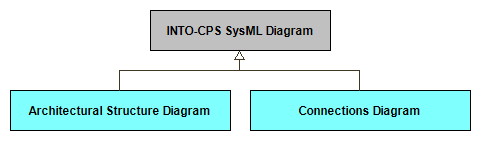
\includegraphics[scale=0.6]{figures/Architecting/ArchitecturalViews}
\caption{Diagrams in the multi-modelling SysML profile}
\label{fig:sysml:intocps}
\end{figure}

\newpage
\subsection{Architectural Structure Diagram}
\label{sec:sysml:intocps:asd}

The \emph{Architecture Structure Diagram} (ASD) specialises SysML block definition diagrams (BDDs) to support the specification of a multi-model architecture described in terms of a systems components, which will be represented by FMUs. As shown in Figure~\ref{fig:sysml:sysml:intocps:ase} this diagram must include a \texttt{<<System>>} which is then broken down into zero or more \texttt{<<Component>>} blocks.

\begin{figure}[h!]
\centering
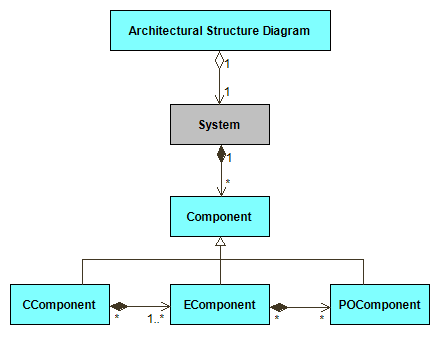
\includegraphics[scale=0.6]{figures/Architecting/ArchitecturalStructureElements}
\caption{\emph{Architectural Structure Diagram} describing FMUs (EComponents) and their hierarchies}
\label{fig:sysml:sysml:intocps:ase}
\end{figure}

There are three types of component block. The \texttt{<<EComponent>>} (encapsulating component) represents a part of a system that will be represented by a single FMU. These blocks have properties indicating which modelling language and tool will be used: \texttt{modelType} (\emph{discrete} or \emph{continuous}) and \texttt{platform} (\emph{VDMRT}, \emph{TwentySim}, \emph{OM}, and \emph{other}).

An \texttt{<<EComponent>>} can be broken down logically into \texttt{<<PComponent>>} (part-of component) representing an internal element of an \texttt{<<EComponent>>}. Both \texttt{<<EComponent>>} and \texttt{<<PComponent>>} blocks can define \emph{variables} and \emph{FlowPorts} that an FMU will have.

The third type of component is a \texttt{<<CComponent>>} (collection component) that allows other components to be grouped logically (it has no ports or behaviours). These can be used to separate design elements within a diagram, as described in Section~\ref{sec:sysml:non-design}. All component blocks have a \emph{kind} that marks their purpose in the model (\emph{cyber}, \emph{physical}, \emph{environment}, \emph{visualisation}).

FMUs are connected by \emph{ports}, and may also present internal state through externally visible \emph{variables}, which can be monitored on a live graph, for example. Both \texttt{<<EComponent>>} and \texttt{<<PComponent>>} blocks can define \emph{FlowPort} and \emph{Variable} attributes, as shown in Figure~\ref{fig:sysml:sysml:intocps:asi}, which will form the interface of the FMU and are added to the ``model description'' exported by Modelio.

\begin{figure}[h!]
\centering
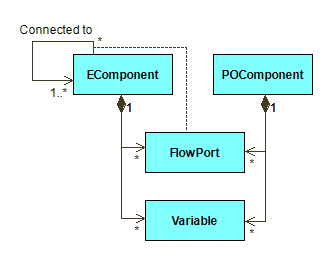
\includegraphics[scale=0.6]{figures/Architecting/ArchitecturalStructureInterfaces}
\caption{Component blocks may define variables and ports}
\label{fig:sysml:sysml:intocps:asi}
\end{figure}

%\begin{figure}[h!]
%\centering
%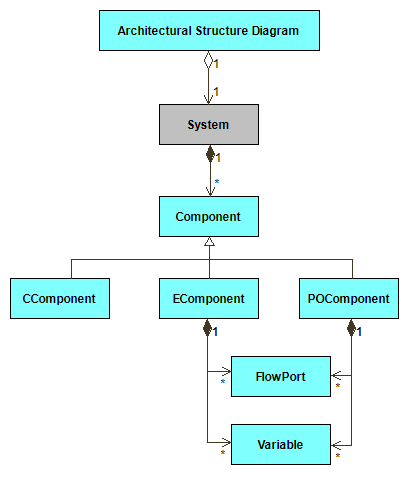
\includegraphics[scale=0.6]{figures/Architecting/ArchitecturalStructureView}
%\caption{\emph{Architectural Structure Diagram} describing connections between FMUs}
%\label{fig:sysml:sysml:intocps:asd}
%\end{figure}

%\clearpage
\subsection{Connections Diagram}
\label{sec:sysml:intocps:cd}

The \emph{Connections Diagram} (CD) specialises SysML internal block diagrams to convey the internal configuration of the systems components. Specifically, it describes which FMUs are instantiated (i.e. which \texttt{<<EComponent>>}s form the ASD), and how the ports are connected. This diagram is used by Modelio to generate multi-model configurations.

\begin{figure}[h!]
\centering
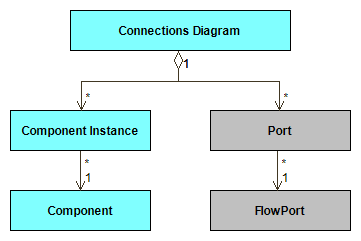
\includegraphics[scale=0.6]{figures/Architecting/ConnectionsView}
\caption{\emph{Connections Diagram} describing the static structure of FMUs}
\label{fig:sysmlintocps:cd}
\end{figure}

\section{SysML Diagrams Describing Design Space Exploration}
\label{sec:sysml:dse}

The design space exploration (DSE) SysML profile is an addition to the multi-modelling SysML profile described above. As with single co-simulation, the INTO-CPS Application can run a DSE based on a JSON configuration file. These can be created manually in a text editor or edited in the INTO-CPS Application. Alternatively, a configuration can be generated by Modelio, from a set of diagrams defined in the profile. There are five diagram types, which are described below. Further guidance on DSE can be found in Chapter~\ref{sec:dse}.

\begin{figure}[h!]
\centering
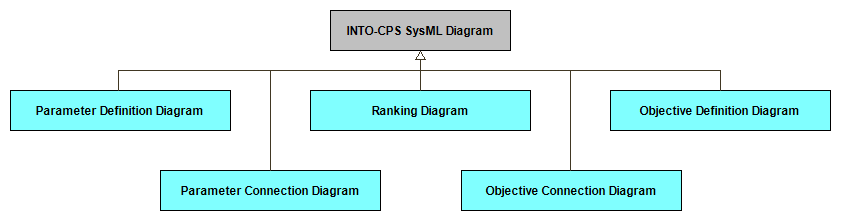
\includegraphics[scale=0.5]{figures/DSE/DSEViews}
\caption{Diagrams in the DSE SysML profile}
\label{fig:sysml:dse}
\end{figure}

\subsection{Objective Definition Diagram}
\label{sec:sysml:dse:odd}

The \emph{Objective Definition Diagram} is used to define the objectives for use during a DSE. Objectives are characterising measures of performance that may be used to determine the relative benefits of competing designs. They are defined as metrics over the results of a co-simulation of a specific design and are used to judge its quality for use in later processing e.g. ranking.

Objectives are described in terms of a name, a script file that will be used to compute them, and the ports that will provide the data they require. As with the \emph{Architectural Structure Diagram} above (Section~\ref{sec:sysml:intocps:asd}), this diagram gives the static structure of the objectives; instances of these definitions are created using the \emph{Objective Connection Diagram} below (Section~\ref{sec:sysml:dse:ocd}).

\begin{figure}[h!]
\centering
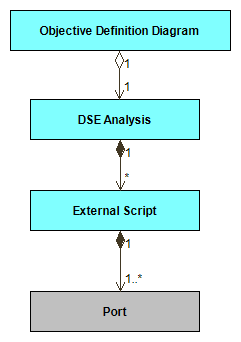
\includegraphics[scale=0.5]{figures/DSE/ObjectiveDefinitionView}
\caption{\emph{Objective Definition Diagram} describing objectives in a DSE}
\label{fig:sysml:sysml:dse:odd}
\end{figure}

\subsection{Objective Connection Diagram}
\label{sec:sysml:dse:ocd}

The \emph{Objective Connection Diagram} is used to instantiate objectives defined in the \emph{Objective Definition Diagram} above (Section~\ref{sec:sysml:dse:odd}). The diagrams allow the ports of each instance of the objective to be linked to a data source: either a static value, or a value from data exchanged in the multi-model.

\begin{figure}[h!]
\centering
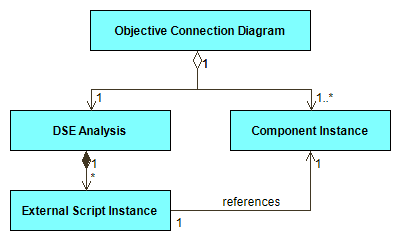
\includegraphics[scale=0.5]{figures/DSE/ObjectiveConnectionsView}
\caption{\emph{Objective Connections Diagram} linking objectives to data sources}
\label{fig:sysml:sysml:dse:ocd}
\end{figure}

\subsection{Parameter Definition Diagram}
\label{sec:sysml:dse:pdd}

The \emph{Parameter Definition Diagram} is used to define the parameters that will changed for each co-simulation in a DSE. Parameters are described in terms of a name, and a set of values that we wish to test. The product of the cardinalities of the set of values for each parameter gives the size of the design space--- the total number of simulation required for an exhaustive search. As with the \emph{Architectural Structure Diagram} above (Section~\ref{sec:sysml:intocps:asd}), this diagram gives the static structure of the parameters; instances of these definitions are created using the \emph{Parameter Connection Diagram} below (Section~\ref{sec:sysml:dse:pcd}).

\begin{figure}[h!]
\centering
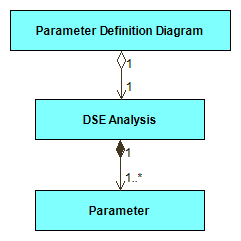
\includegraphics[scale=0.5]{figures/DSE/ParameterDefinitionView}
\caption{\emph{Parameter Definition Diagram} defining parameters and their values}
\label{fig:sysml:sysml:dse:pdd}
\end{figure}

\subsection{Parameter Connection Diagram}
\label{sec:sysml:dse:pcd}

The \emph{Parameter Connection Diagram} is used to instantiate parameters defined in the \emph{Parameter Definition Diagram} above (Section~\ref{sec:sysml:dse:pdd}). The diagram allows the parameters to be linked to those provided by the FMUs in the multi-model.

\begin{figure}[h!]
\centering
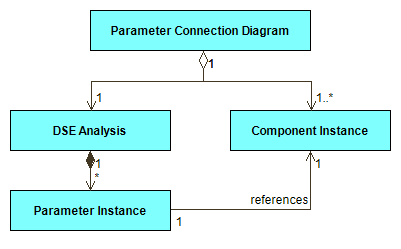
\includegraphics[scale=0.5]{figures/DSE/ParameterConnectionsView}
\caption{\emph{Parameter Connections Diagram} linking parameters to FMUs}
\label{fig:sysml:sysml:dse:pcd}
\end{figure}

\subsection{Ranking Diagram}
\label{sec:sysml:dse:rd}

The \emph{Ranking Diagram} is used to declare which of the objectives should be used to compare competing designs, and whether lower or higher values for each the objectives is better (i.e. whether to maximise or minimise a value).

\begin{figure}[h!]
\centering
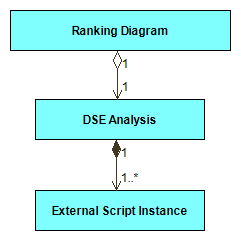
\includegraphics[scale=0.5]{figures/DSE/RankingView}
\caption{\emph{Ranking Diagram} defining how to rank designs based on objectives}
\label{fig:sysml:sysml:dse:rd}
\end{figure}


\section{Holistic and Design Architectural Modelling}
\label{sec:sysml:holistic}

A system architecture defines the major components of a system, and identifies their relationships, behaviour and interactions. A model of the architecture is potentially partial (representing some or all of the system) and abstract, limited to those elements pertinent to the modelling goal. In CPS engineering, this goal may include understanding the system in terms of the application domain (a \emph{holistic} model), or capturing the system components in a way that targets multi-modelling (a \emph{design} model).

The diagrams in the two profiles described above divide architectural models into subsystems composed of cyber or physical components. Defining an architecture this way may not be the best approach when designing a system ab initio, with systems comprising entities across different domains requiring diverse domain expertise. Following on from Chapter~\ref{sec:reqeng}, this section uses a smart grid example to show both holistic and design architectural modelling approaches, and provide some commentary and guidance on how to model in a way which is natural for domain experts, and how to move from holistic to design models when multi-modelling.

\subsection*{Example Introduction}

%\fbox{mention what a SG is briefly:  control, distributed control, ideas of power gen, transmission, substations etc}
A smart grid is an electricity power grid where integrated ICT systems play a role in the control and management of the electricity power supply. Such ICT elements include distributed control in households, control of renewable energies and networked communications.
In this section we outline a Smart Grid\ model to explore different design decisions in the cyber control of an electricity power grid. The model presented here is a small illustrative example, which omits complexities of a real Smart Grid. For example, the change from three-phase AC power to one-phase DC power allowing us to use simpler physical models. A second simplification is in the number of houses present in the grid model. We model only 5 houses, assumed to be in a small local area supplied by a single substation. We do not consider the remainder of the grid. To ensure that any effect due to changes in the power consumption by those properties are observed by the other houses, we skew the resistance of the transmission lines between the power generation and substation, and substation to houses.

\subsection*{Holistic Architectural Model}

A Block Definition Diagram (BDD) of the Smart Grid is given in Figure~\ref{fig:bdd}. The figure shows that the \textit{Smart Grid} system comprises two top-level physical elements: \textit{Power Generation} and \textit{Transmission Lines}; a single top-level cyber elements: the \textit{Data Network}; and two cyber-physical systems: a \textit{Substation} and several \textit{Houses}. The two elements may be further decomposed. The \textit{Substation} elements is composed of a cyber \textit{Substation Controller} and physical \textit{Substation Meter} and \textit{Step-down Transformer}. The \textit{House} element comprises: a cyber \textit{House Controller}, physical \textit{House Meter} and \textit{Devices}, and an \textit{Owner/Usage Profile}.

\begin{figure}
\centering
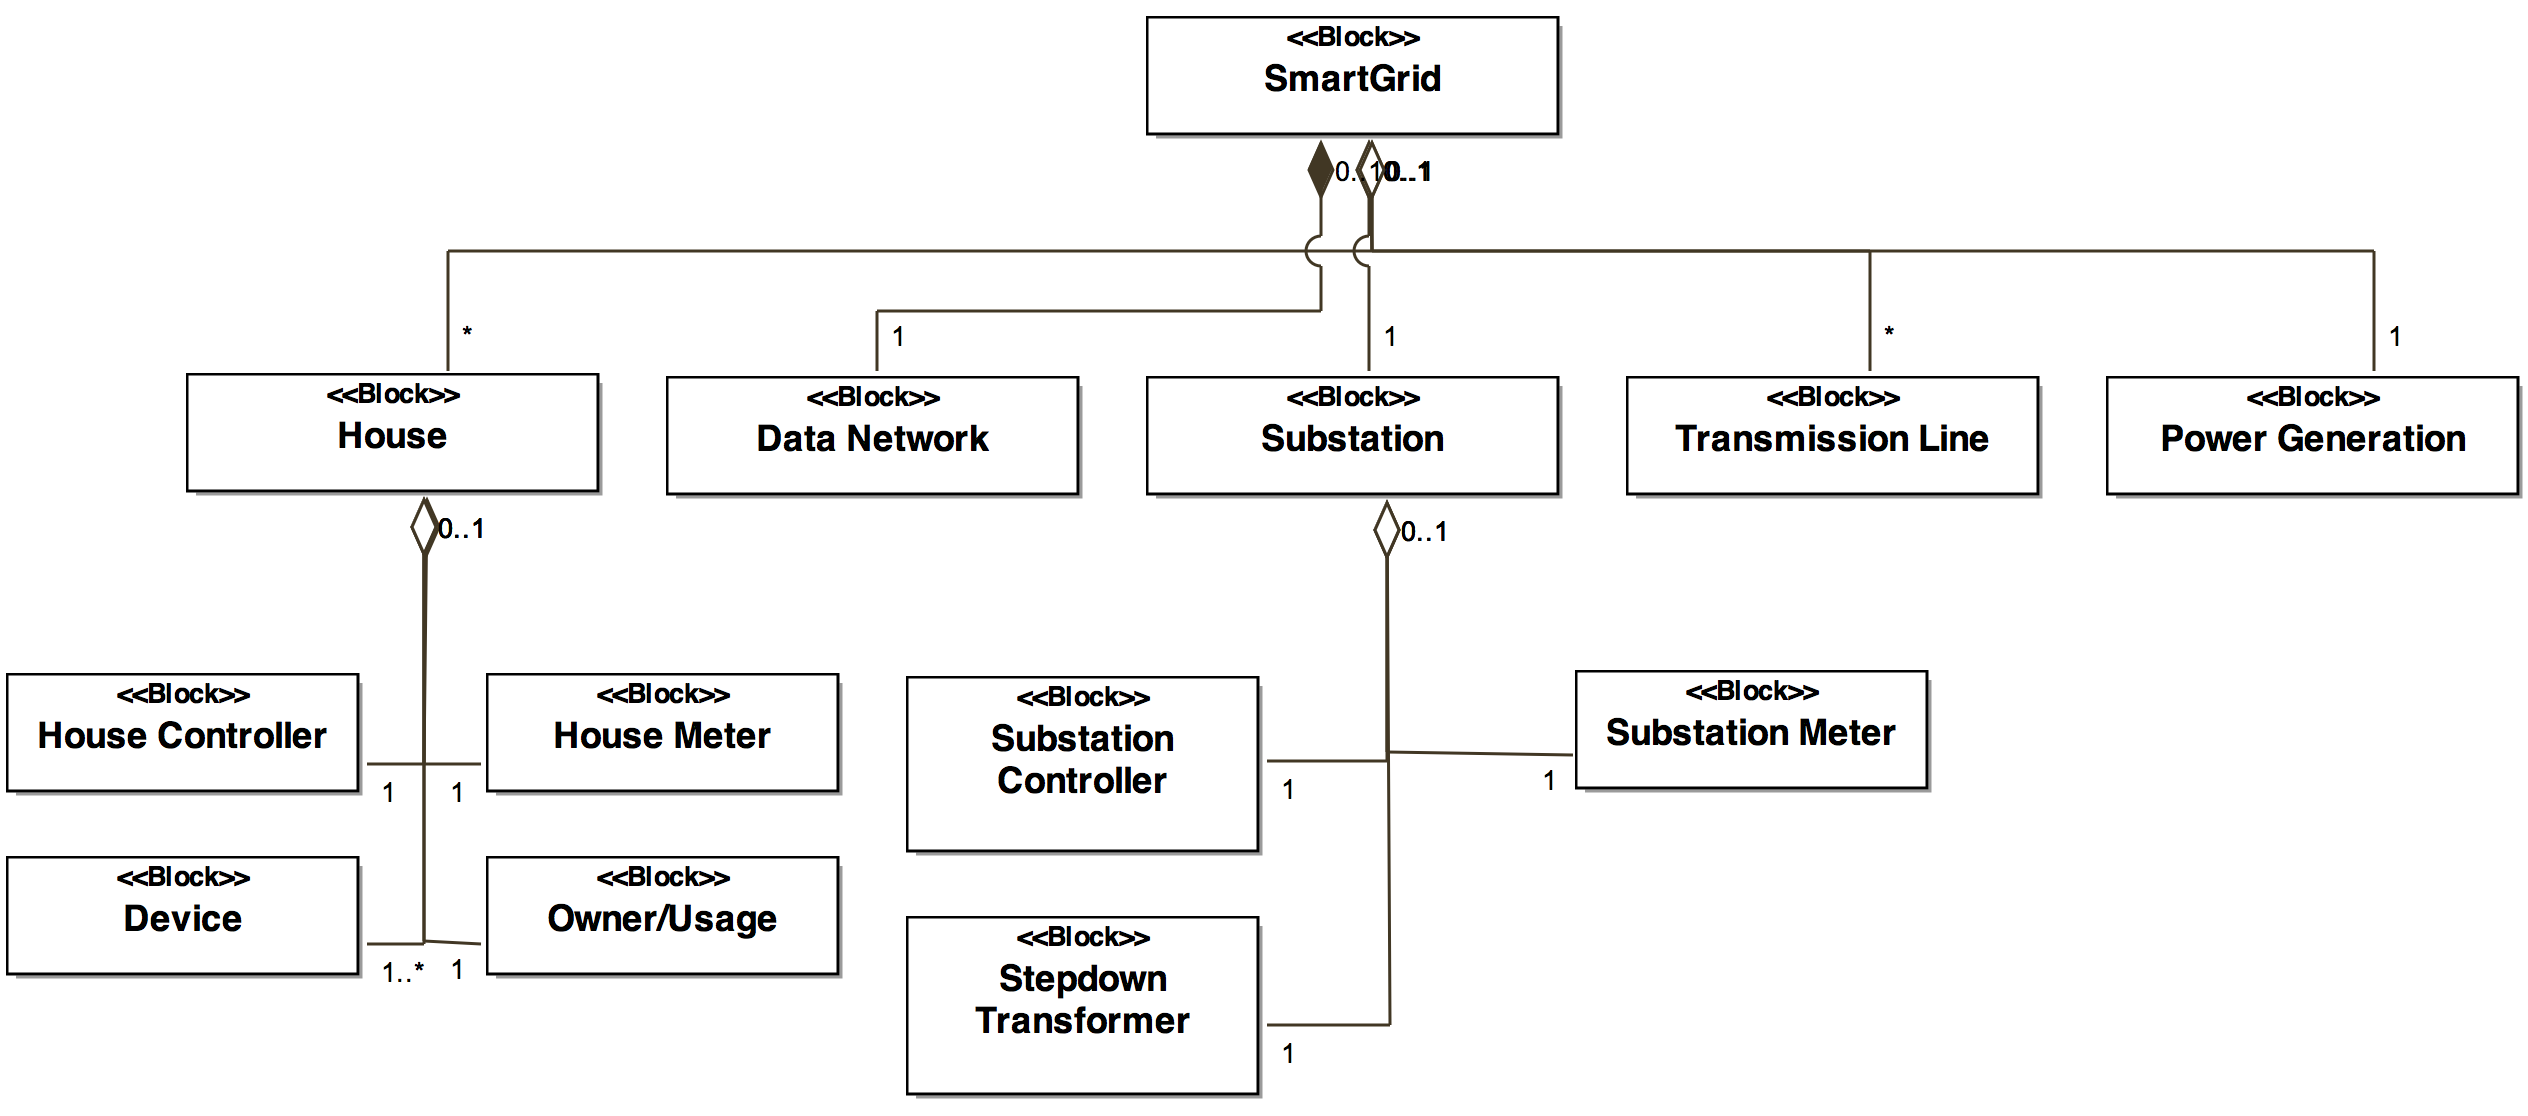
\includegraphics[width=1\textwidth]{figures/BDDSmartGrid}
\caption{Block Definition Diagram of Smart Grid}
\label{fig:bdd}
\end{figure}

An Internal Block Diagram (IBD) of the Smart Grid is given in Figure~\ref{fig:ibd}. The diagram shows there are two main connection types in the model, corresponding to the physical power connections and the cyber data connections. The model also shows the connections between the cyber and physical parts of the models -- currently modelled using data-type connections.

\begin{figure}
\centering
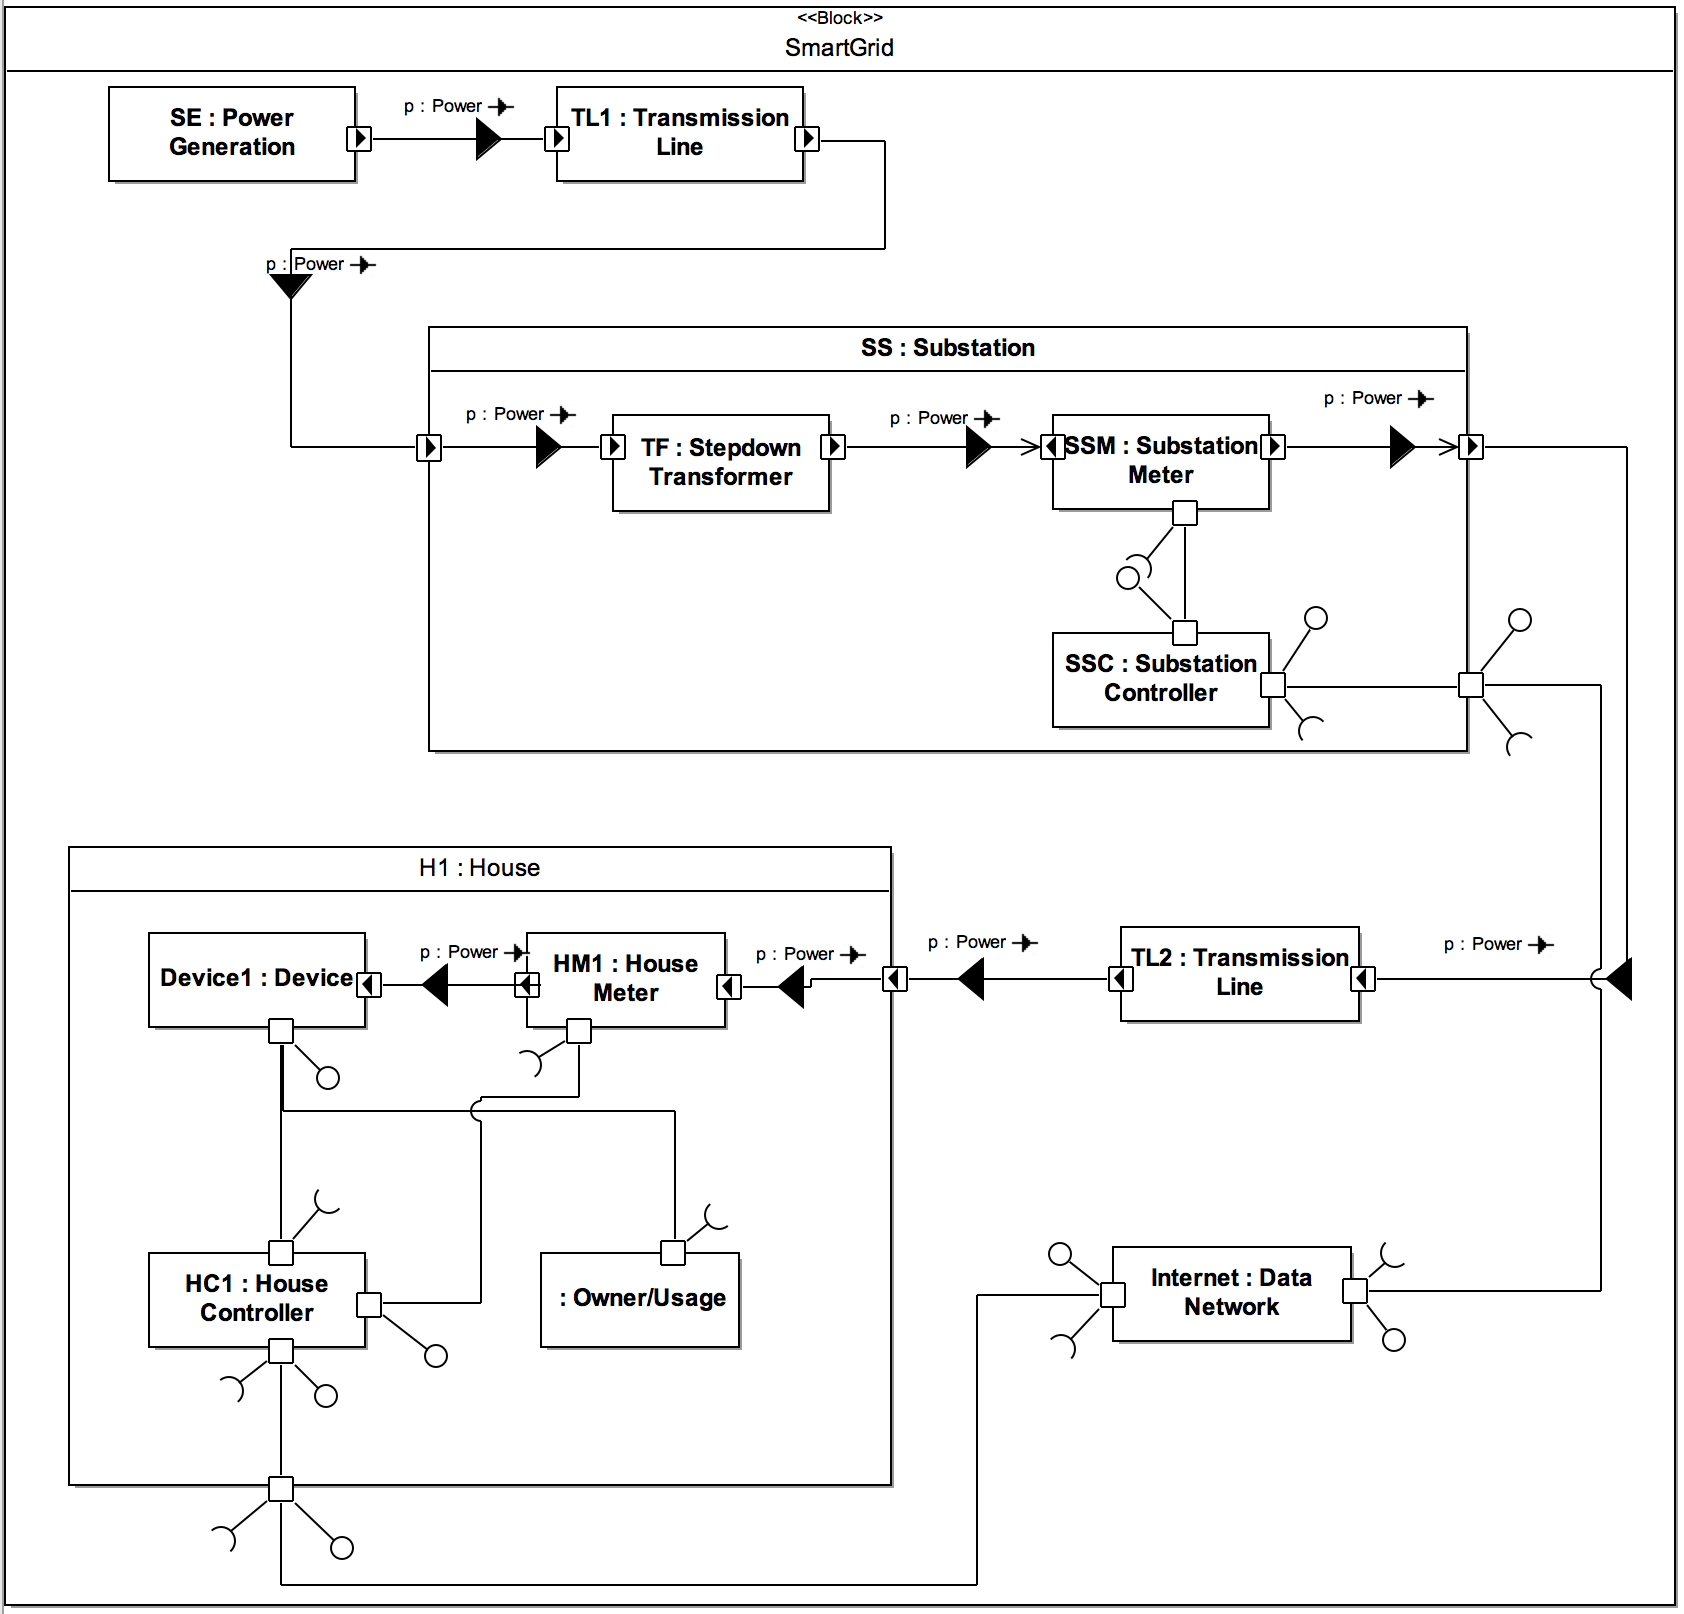
\includegraphics[width=0.85\textwidth]{figures/IBDSmartGrid}
\caption{Internal Block Diagram of Smart Grid}
\label{fig:ibd}
\end{figure}

The first type of connection ---the physical power connections--- show a flow of \textit{Power} from the Power Generation, through the Transmission Lines to the Houses, via the Substation. In the Substation, the Stepdown Transformer is connected to the Substation Meter. Similarly, in each House (only one is shown in the figure), the Power flows through the House Meter to each Device (again only one is shown for readability). The data connections exist between the Substation Controller and House Controllers. The Data Network is explicitly modelled and links the various controllers. Finally, there are links between the cyber controllers and the physical systems. In this model, the Substation Controller is connected to the Substation Meter, and the House Controller is linked to the House Meter and Devices.

\subsubsection*{Design Architectural Model}

% KGP: So actually we could update this to use CComponents to ``better reflect the holistic architecture''?

Looking at the holistic architecture defined in Figures~\ref{fig:bdd} and~\ref{fig:ibd} and moving towards a multi-model, we use the INTO-CPS SysML profile to define the architecture of the Smart Grid\ from the perspective of multi-model. This yields the ASD in Figure~\ref{fig:asd_mm}. This structure removes all subsystem structures such that each component is to be realised in a single FMU. Each element is defined as either a \emph{physical} or \emph{cyber} component, with the model type and platform identified.

\begin{figure}[htbp]
\centering
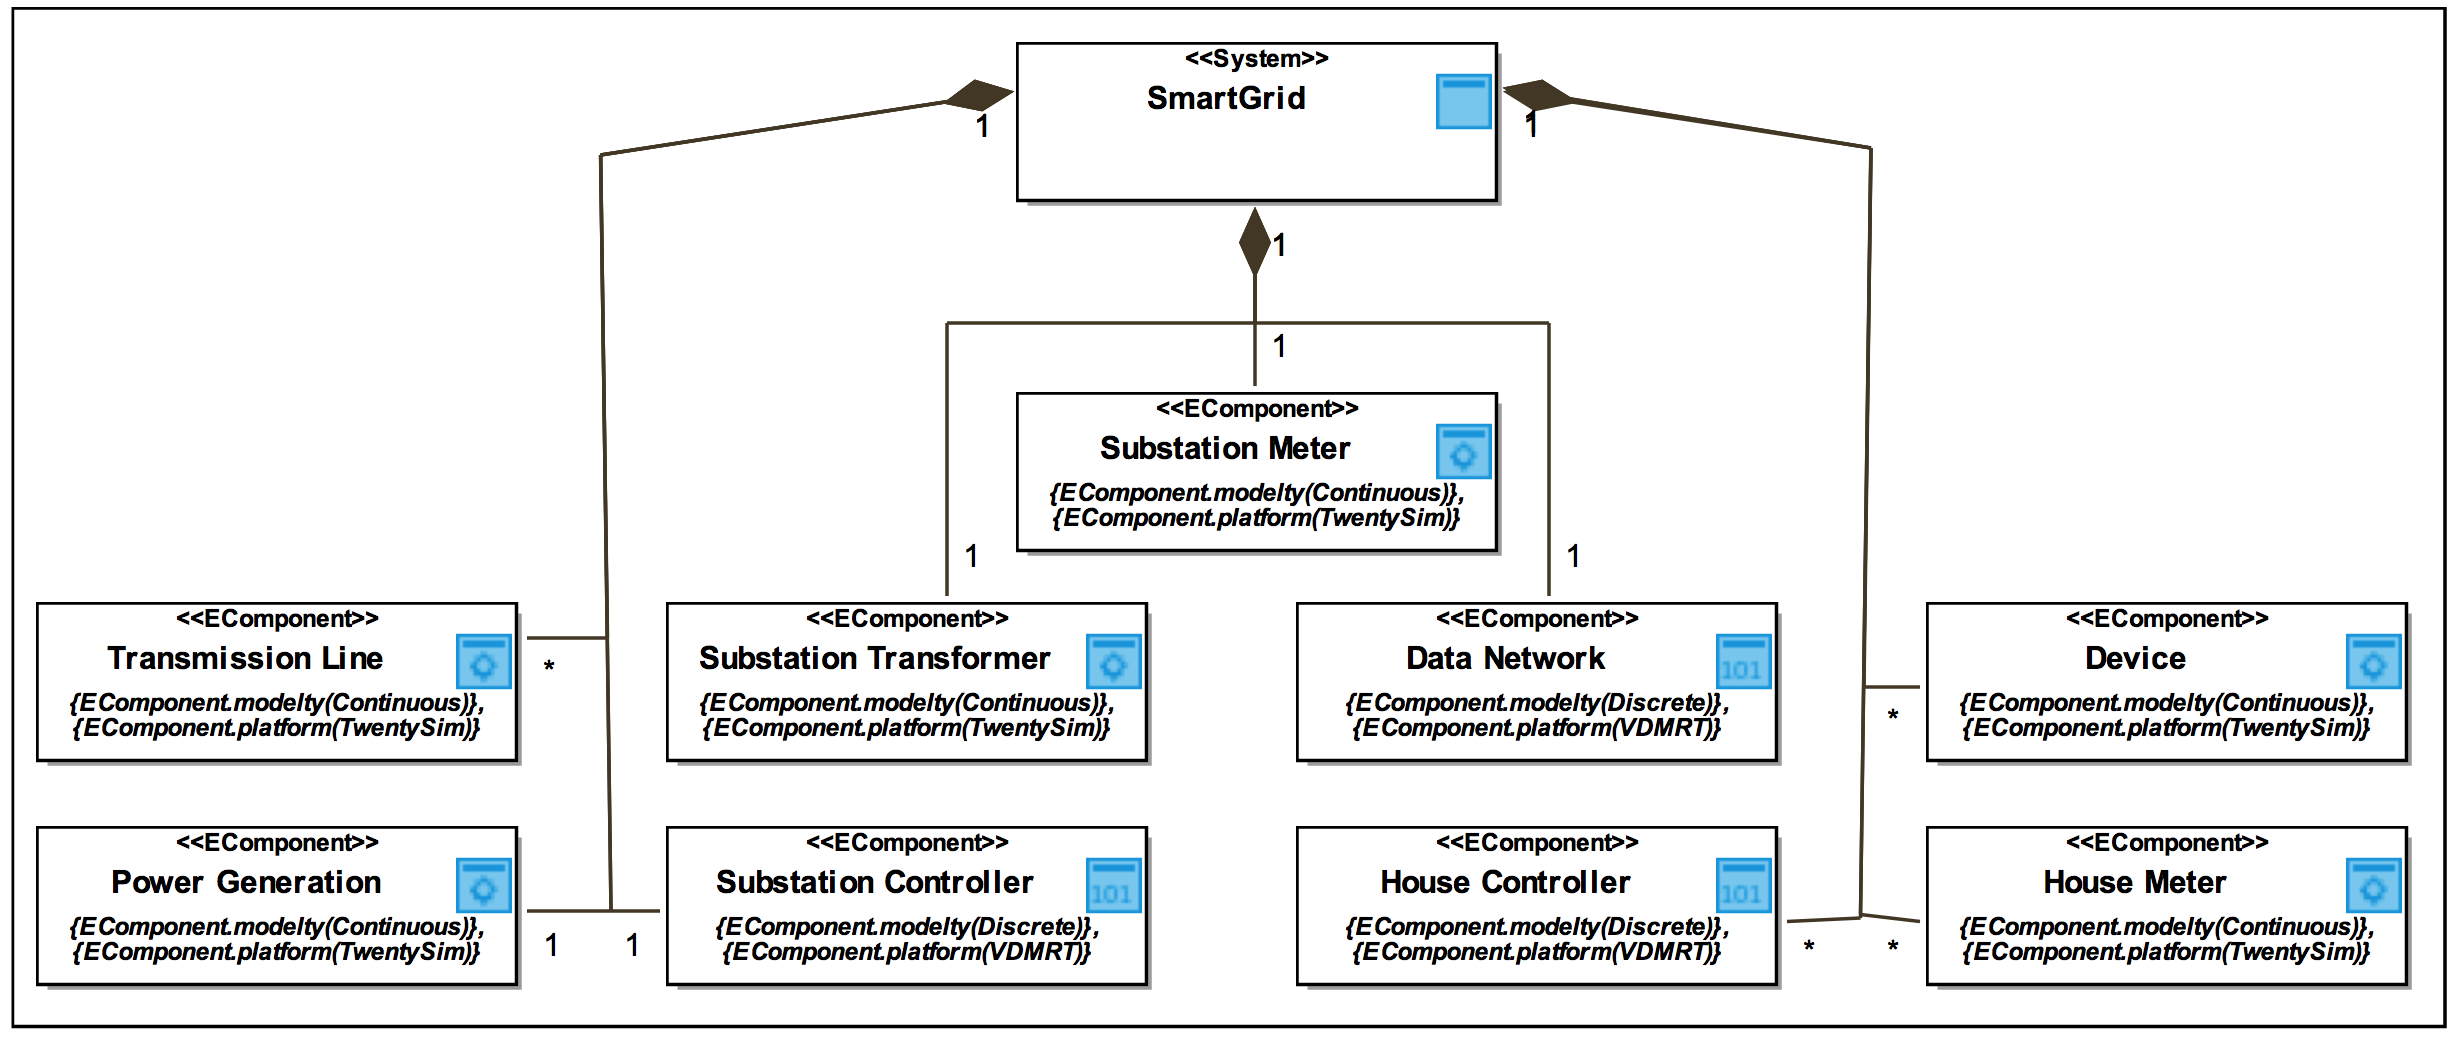
\includegraphics[width=0.9\textwidth]{figures/ASD_mm}
\caption{Architecture Structure Diagram for multi-model of Smart Grid}
\label{fig:asd_mm}
\end{figure}

The connections between the components are defined in the Connections Diagram (CD) in Figure~\ref{fig:cd_mm}. The interface between subsystems is defined as the interaction points between cyber and physical components (FMUs).

\begin{figure}
\centering
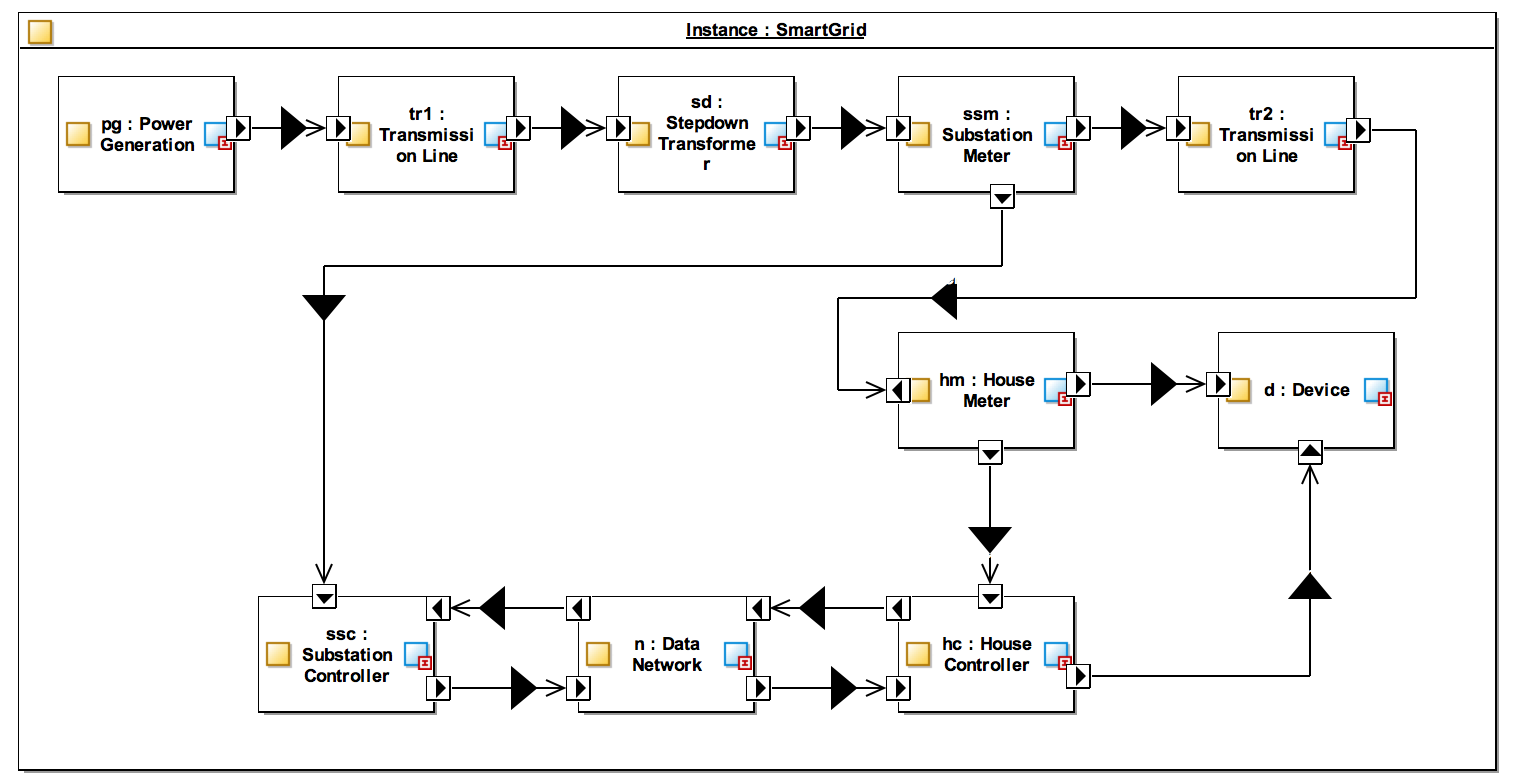
\includegraphics[width=1\textwidth]{figures/CD_mm}
\caption{Connections Diagram for multi-model of Smart Grid}
\label{fig:cd_mm}
\end{figure}

\subsubsection*{Discussion}

Contrasting the architectures shown in the initial model (Figures~\ref{fig:bdd} and~\ref{fig:ibd}) to that in the multi-model (Figures~\ref{fig:asd_mm} and~\ref{fig:cd_mm}), whilst the same base components are present in both, some of the intuitive domain-specific structures are lost when moving to a multi-model. For example, it is now not clear where the \emph{substation} or \emph{house} elements are in the multi-model.

An important issue here is in the reason behind producing different architectural models. Using SysML diagrams in a \emph{holistic} approach, a CPS engineer describes the model using a structure natural to the application domain. As such, the \emph{reason} for modelling is not in the ultimate analysis to perform, but to define and understand the structure and behaviour of a system. In contrast, the \emph{design} approach is necessary to configure INTO-CPS multi-models from SysML.

Figure~\ref{fig:sysml_mm} presents an overview of the relationships between the different types of models. The figure shows that the `real' system may be modelled in different forms: the holistic and design architectures and the multi-model.

\begin{figure}
\centering
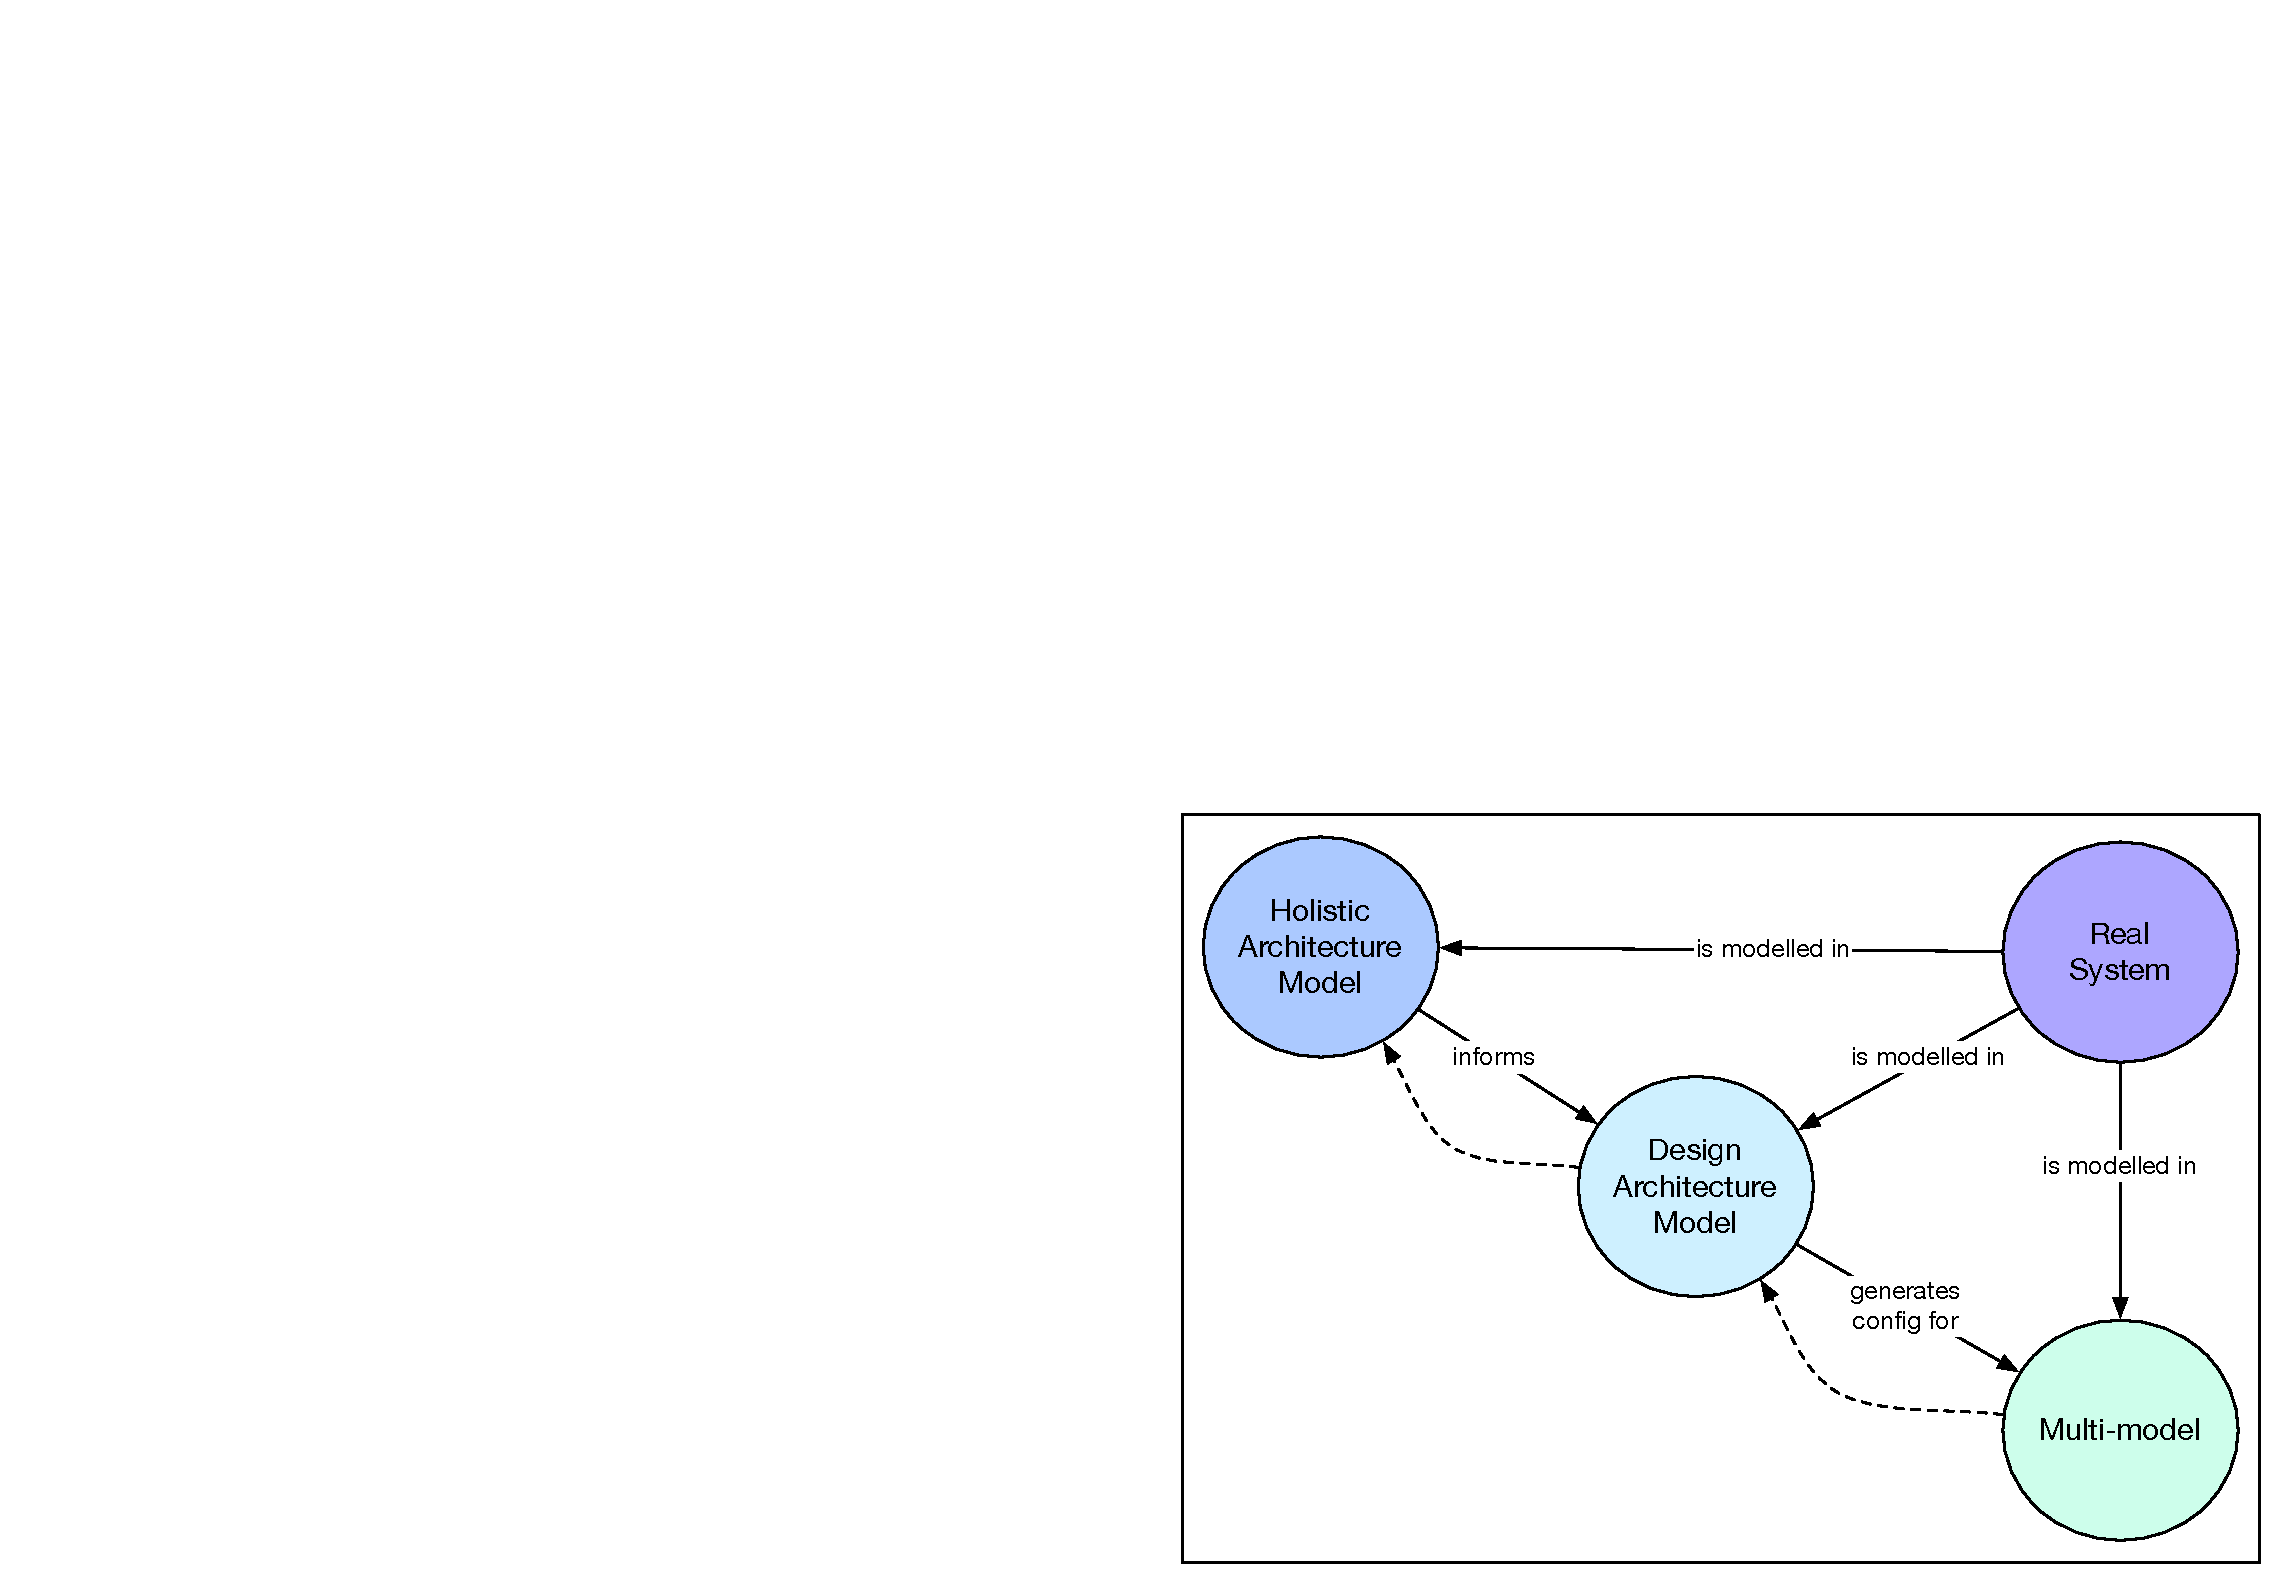
\includegraphics[width=0.7\textwidth]{figures/sysml_for_mm}
\caption{Relating holistic and design architectures}
\label{fig:sysml_mm}
\end{figure}

As illustrated in the figure, one approach can inform another. In some cases this may be a natural process; for example in the Smart Grid\ example, isolating each of the lowest level components in Figure~\ref{fig:bdd} to be individual FMUs in a multi-model is an evolution which will likely result in a feasible model. By creating a domain-specific holistic architecture first, then transforming these models into a design architecture for multi-modelling, design teams will likely gain the most benefit.


\section{Representing Non-Design Elements in SysML}
\label{sec:sysml:non-design}

Using the INTO-CPS tool chain, we generate co-simulation configurations using an architectural model defined with the INTO-SysML profile. This model defines the structure of a system in terms of the composition of its components and their connections. There are however circumstances where elements in the multi-model are not part of the design of the final system, for example where an FMU is used purely for visualisation. This FMU must be connected to the system components, however is not itself a system component. This is also true when considering the environment of the system.

Here we present a small example of the use of these extensions, using a simple robot example (based on the line-following robot pilot study, see Deliverable D3.6~\cite{INTOCPSD3.6}) to illustrate the use of \texttt{<<CComponent>>}s and the \emph{kind} of components (\emph{cyber}, \emph{physical}, \emph{environment}, \emph{visualisation}) described in Section~\ref{sec:sysml:intocps:asd} above.

The architecture structure diagram in Figure~\ref{fig:example_asd} shows: a \emph{System\_Env} block, an \texttt{<<EComponent>>} defined as an \texttt{Environment} FMU; a \emph{3D\_View} block an \texttt{<<EComponent>>}, defined as an \texttt{Visualisation} FMU; and an \emph{Example\_Robot} block, an \texttt{<<EComponent>>} defined as an \texttt{composition} of two FMUs.

\begin{figure}
\centering
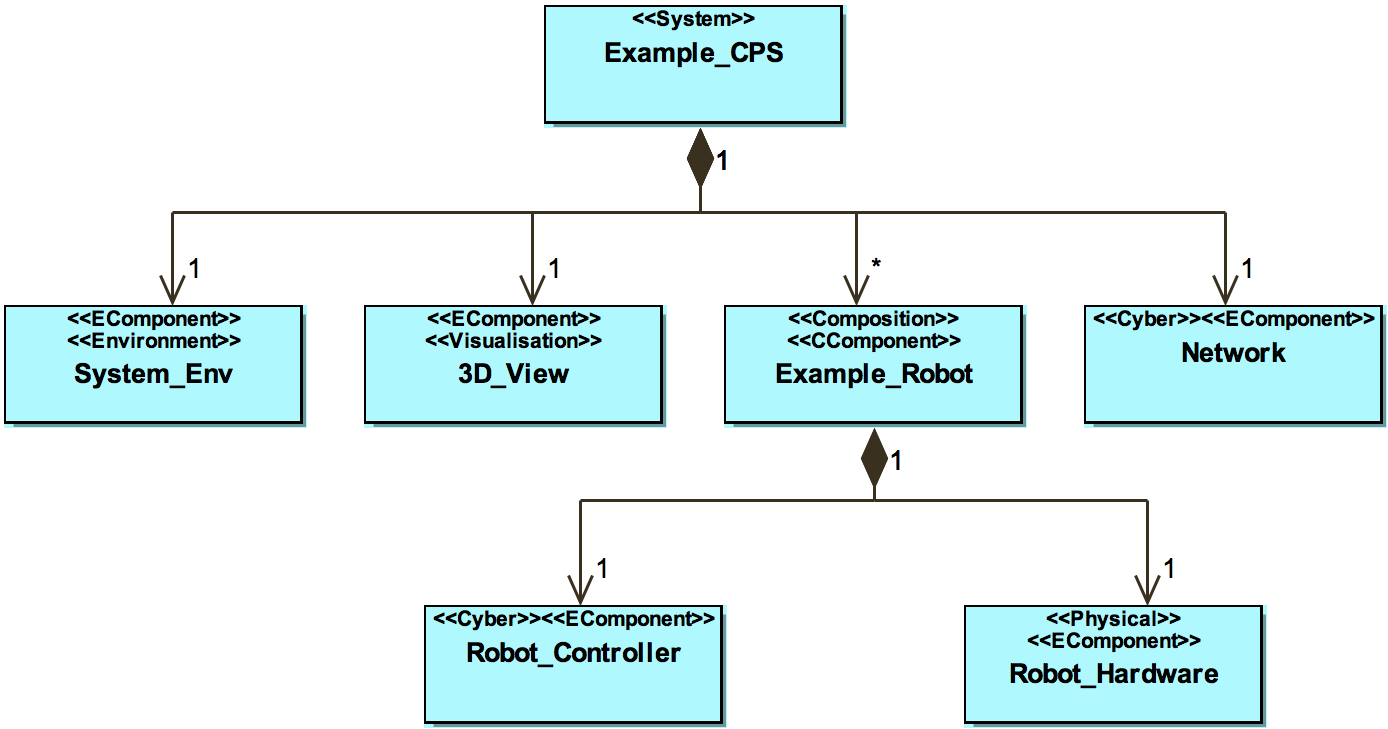
\includegraphics[width=0.8\textwidth]{figures/E_Blocks_ext_asd}
\caption{Example Architecture Structure Diagram of robot system}
\label{fig:example_asd}
\end{figure}

The example has two connection diagrams. The first is shown in Figure~\ref{fig:example_cd}, it contains only those connections with respect to the system and its constituent components . This diagram shows a block instance \emph{cps1} containing the environment (\emph{e}) and the example robot (\emph{r}) which  contains two the controller and hardware components.

The second is shown in Figure~\ref{fig:example_cd2}, it depicts the use of the block instance \emph{3D} of type \emph{3D\_View}. In this diagram, we show additional ports of the original block instances to output internal model details and connect these to the \emph{3D} instance. The diagram includes the system connectors as shown in Figure~\ref{fig:example_cd}.

\begin{figure}
\centering
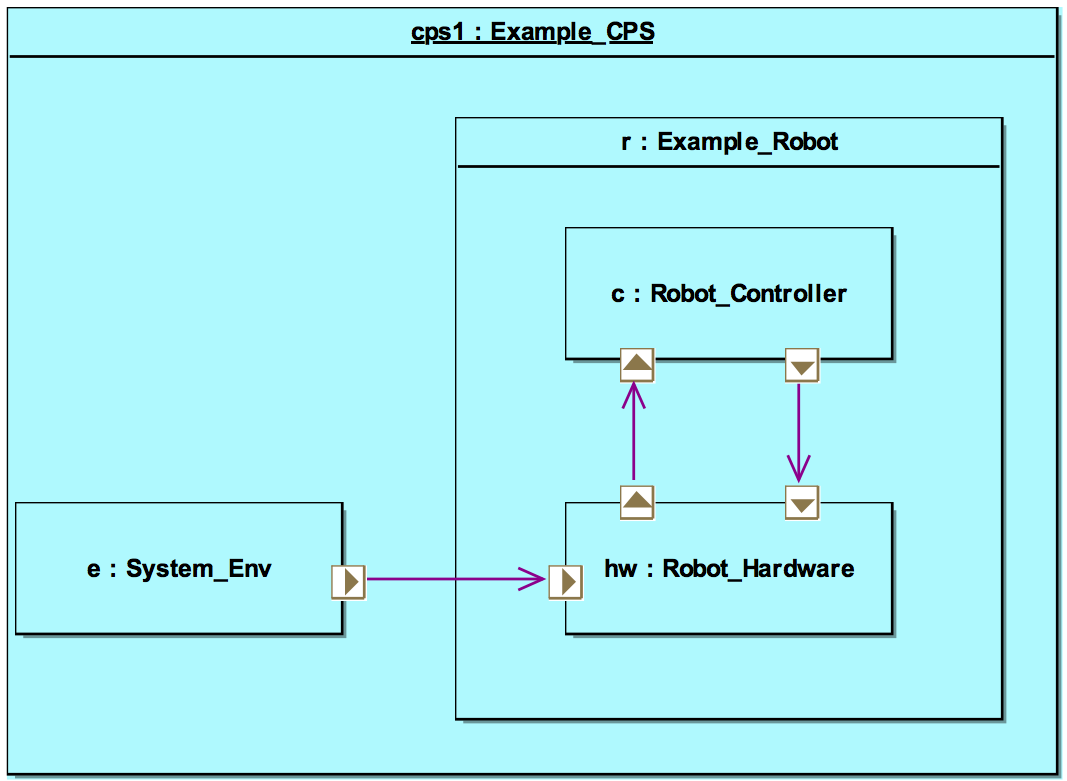
\includegraphics[width=0.6\textwidth]{figures/E_Blocks_ext_cd}
\caption{Connections Diagram for robot showing only system and environment connectors}
\label{fig:example_cd}
\end{figure}

\begin{figure}
\centering
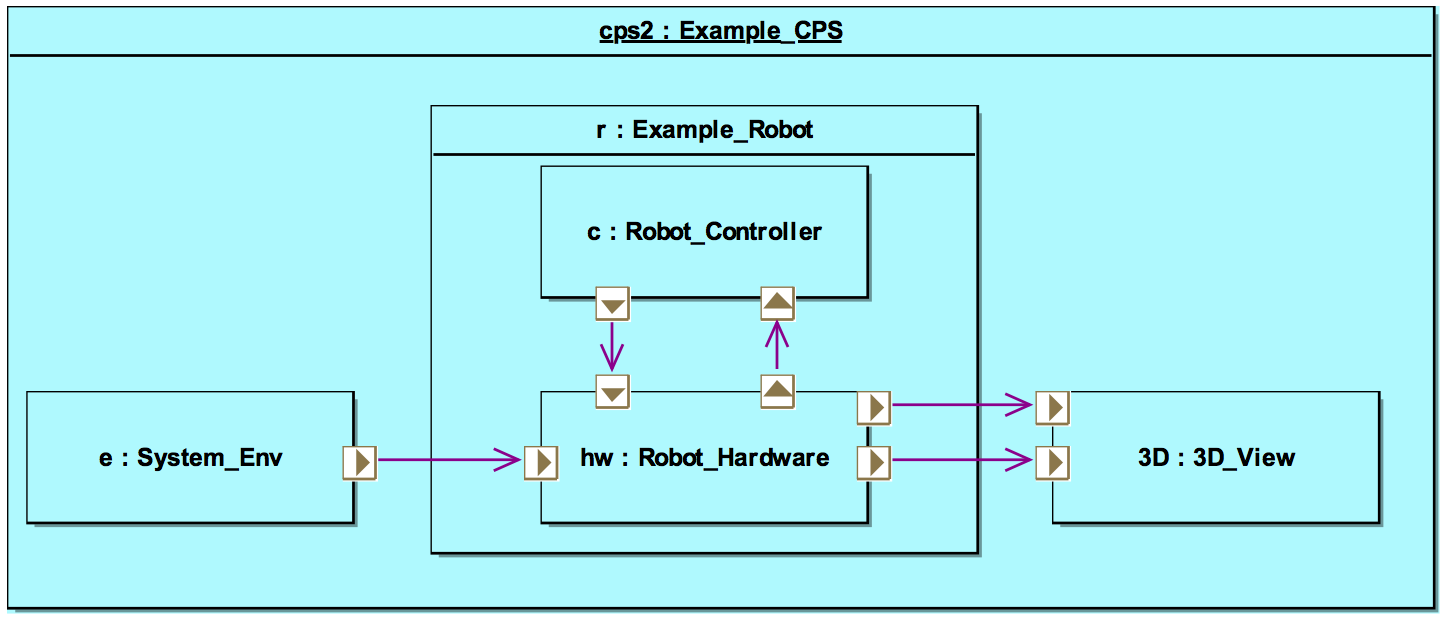
\includegraphics[width=0.9\textwidth]{figures/E_Blocks_ext_cd2}
\caption{Connections Diagram for the robot system showing the system \textit{and} visualisation components}
\label{fig:example_cd2}
\end{figure}










%
% MOVED TO D4.2c
%

%\section{Metamodel and Profile Extensions}
%
%As such, we have extended the INTO-CPS SysML metamodel and profile to allow a multi-model to include an FMU for visualisation and the environment, the addition of the CComponents type and an extension for FlowPorts to support minimum and maximum values in later versions of the SysML-FMI translation.
%
%In this document we present the extensions to INTO-SysML first in metamodel fragments (Figure~\ref{fig:mm-extensions}) and then as SysML profile diagrams (Figure~\ref{fig:profile-extensions}), as presented in~\cite{INTOCPSD2.1a}. In Figure~\ref{fig:fblocks_ext}, we extend the F\_Blocks metamodel fragment to include CComponents, additional ComponentKind enumerations and the repositioning of Flowport ownership -- changes are shown in red. The diagram shows that a \texttt{CComponent} is a subtype of \texttt{Component}, and contains no additional attributes. To support modelling of non-CPS components, three extra \texttt{ComponentKind} enumerations are added: \texttt{environment}, \texttt{visualisation} and \texttt{composition}. Finally, where previously the \texttt{Block} stereotype was the owner of \texttt{FlowPorts}, we have adjusted that relationships so that neither \texttt{System} or \texttt{CComponent} instances can own \texttt{FlowPorts}.
%
%A minor update to the \texttt{FlowPort} definition is shown in Figure~\ref{fig:port_ext}. The extension is to allow minimum and maximum values for flowports to be defined. The \texttt{min} and \texttt{max} attributes are of type PType -- the primitive types of INTO-SysML.
%
%\begin{figure}[htbp]
%\begin{center}
%\subfigure[Extension to F\_Blocks fragment]
%{
%	\includegraphics[width=0.5\textwidth]{figures/MM_Blocks}
%	\label{fig:fblocks_ext}
%}
%\subfigure[Extension to F\_Props fragment]
%{
%	\includegraphics[width=0.4\textwidth]{figures/MM_Ports}
%	\label{fig:port_ext}
%}
%\caption{Extended Metamodel fragments of INTO-SysML -- extensions are highlighted with a red dotted line.}
%\label{fig:mm-extensions}
%\end{center}
%\end{figure}
%
%The next collection of figures present the extensions to the INTO-SysML profile, which implement the above metamodel extensions. Figure~\ref{fig:profile-blocks-comp} realises the composition aspect of F\_Blocks metamodel fragment in Figure~\ref{fig:fblocks_ext}. Two extensions are defined: firstly a specialisation of the \texttt{Component} stereotype, \texttt{CComponent} is defined; and secondly the three additional options for the \texttt{ComponentKind} enumeration are defined.
%
%Figure~\ref{fig:profile-blocks-conn} presents a realisation of the F\_Props metamodel in Figure~\ref{fig:port_ext}, and the reorganisation of FlowPort ownership from the F\_Blocks metamodel fragment in Figure~\ref{fig:fblocks_ext}. Two main changes are defined. The first, adds two new tags to the \texttt{FlowPort} stereotype -- \texttt{min} and \texttt{max}. The second change is the adjustment of flowport ownership. In the original profile a \texttt{Block} may own \texttt{FlowPorts}, we have changed this to reflect the metamodel and so the \texttt{EComponent} and \texttt{POComponents}\footnote{A PComponent, as defined in Deliverable D2.1a~\cite{INTOCPSD21a} is an \emph{Part-of Component}, corresponding to an internal element of an encapsulated component.} are the only to \texttt{Block}  specialisations that may own the ports.
%
%\begin{figure}[htbp]
%\begin{center}
%\subfigure[Blocks compositon]
%{
%	\includegraphics[width=0.5\textwidth]{figures/Profile_Blocks1}
%	\label{fig:profile-blocks-comp}
%}
%\subfigure[Blocks connections]
%{
%	\includegraphics[width=0.9\textwidth]{figures/Profile_Blocks2}
%	\label{fig:profile-blocks-conn}
%}
%\caption{Extension to INTO-CPS SysML Profile}
%\label{fig:profile-extensions}
%\end{center}
%\end{figure}
%
%In the next section we provide an example of the use of these extensions.

%\section{Illustrative Example}

